\documentclass[a4paper,10pt]{article}

\usepackage[utf8]{inputenc}
\usepackage{graphicx}

% Path relative to the main .tex file.
\graphicspath{ {./images/} }

\title{Scalavelli project}
\date{25 agosto 2020}
\author{M. Cavalluzzo, L. Giogietti, L. Pagnini, D. Tentoni as "Part Time Team"}

\begin{document}
    \pagenumbering{gobble} % no numbers.
    \maketitle
    \newpage
    \pagenumbering{arabic} % start counting numbers.

    \begin{abstract}
        Progetto scritto in Scala per giocare al celebre gioco Machivelli sul proprio computer e sfidare altri giocatori.
    \end{abstract}

    \tableofcontents

    \newpage


    \section{Processo di sviluppo}

    \subsection{Metodologia}

    Sin da subito abbiamo deciso di adottare una metodologia di sviluppo \textit{Agile-Scrum}, seppur non scegliendo un
    vero e proprio Scrum Master. Chi più e chi meno, a seconda dei vari sprint, praticamente tutti hanno avuto
    l'occasione, il modo e la motivazione di ricoprire tale ruolo, in modo tale da favorire il proseguimento del
    progetto coordinando il team con l'aiuto degli strumenti a disposizione. % Chi è il nostro Scrum Master?
    In accordo con tale metodologia, il lavoro è stato suddiviso in sprint al termine dei quali si sarebbero dovute
    sviluppare un numero minimo di funzionalità dell'applicativo, della durata media di una settimana e mezzo. I meeting
    sono stati frequenti all'inizio e ne sono stati svolti alcuni saltuariamente all'interno di ogni sprint. Questo
    perché, alternandosi con un periodo di lavoro autonomo, abbiamo ritenuto necessario e producente confrontarsi anche
    durante gli sprint su scelte sintattiche e pattern di sviluppo tra tutti i membri del team, in modo da condividere
    conoscenze ed entusiasmo.

    \subsection{Strumenti adottati}
    Come strategia di workflowing è stata scelta questa variante molto semplice, schematizzata di seguito:
    \begin{center}
        \begin{figure}
            \caption{Git workflow.}
            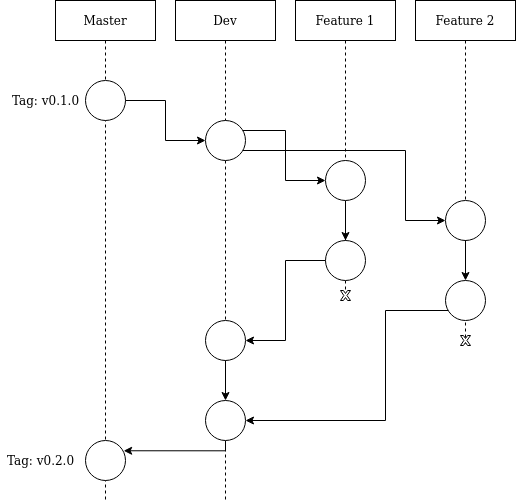
\includegraphics[width=\textwidth, scale=0.8]{git-workflow-1-1.png}
        \end{figure}
    \end{center}
    % TODO: Produrre immagine che rappresenti il workflow.
    Come strumenti di \textit{Build Automation} si è deciso di usare \textit{SBT}, dato che durante il corso lo si è
    sempre preferito rispetto al cugino Gradle per lo svolgimento degli elaborati, nonostante il fatto che alcuni
    componenti del gruppo lo uilizzino in ambito aziendale.
    La comunicazione all'interno del gruppo è avvenuta su \textit{Telegram} per quanto concerne meri aspetti
    organizzativi, mentre la condivisione di appunti e blocchi di codice durante le sessioni di sviluppo è stato
    sfruttato \textit{Microsoft Teams}.
    Per la \textit{Continuous Integration} è stato scelto \textit{Travis CI}. Consisteva nell'unica soluzione freeware
    che i componenti del gruppo abbiano mai usato, introdotta proprio in questo corso. Tuttavia, è stato necessario
    approfondire l'argomento tramite studio autonomo, dato che ciò che si era appreso a lezione è stato ritenuto
    insufficente per la buona riuscita del progetto per come è stato pensato. Ad esso è stata affidata l'esecuzione dei
    test necessari per verificare la correttezza del lavoro svolto e poter poi effettuare dei rilasci senza regressioni.
    Tramite lo stesso servizio, è stata effettuata la \textit{Continuous Delivery}, rilasciando dei pacchetti compilati
    su \textit{Github Releases}.

    \newpage


    \section{Requisiti}\label{sec:requisiti}

    \subsection{Business}\label{subsec:business}

    Il progetto Scalavelli vuole ricreare l’esperienza del celebre gioco di carte Machiavelli in modalità multiplayer,
    tra giocatori differenti locati sulla stessa macchina o nella stessa LAN. Ogni giocatore deve potersi identificare
    con un proprio username e partecipare ad una partita da uno o più giocatori, eventualmente scegliendo di giocare
    specificatamente con i propri amici inserendo il codice identificativo di una partita privata.

    \subsection{Utente}\label{subsec:utente}
    \begin{itemize}
        \item Il giocatore deve poter vedere sullo schermo le combinazioni che ci sono attualmente sul tavolo da gioco,
        le carte che ha in mano, il nome degli altri giocatori e il numero di carte nelle loro mani.
        \item Il giocatore deve poter scegliere il proprio username quando avvia il gioco.
        \item Tramite il proprio username, ci si deve poter registrare presso il server.
        \item Quando viene raggiunto il numero massimo di giocatori per una lobby, allora il server deve subito far
        partire una partita tra i giocatori così riuniti.
        \item Quando un giocatore non risponde più al server per qualche motivo, sia una disconnessione volontaria o un
        problema dell’infrastruttura di rete, la partita finisce immediatamente, venendo visto come un abbandono.

    \end{itemize}

    \subsection{Funzionali}
    \begin{itemize}
        \item Il gioco
        \begin{itemize}
            \item Preparazione del gioco:
            All'inizio della partita devono essere mescolati tra loro due mazzi da 52 carte ognuno (vengono tenuti
            i due Jolly di ogni mazzo). Successivamente vengono distribuite 13 carte ad ogni giocatore.
            \item Svolgimento di un turno:
            Il giocatore di turno può compiere le seguenti azioni:
            \begin{itemize}
                \item Giocare una combinazione:
                \item Aggiungere carte ad una combinazione già esistente
                \item Prendere carte dal tavolo
                \item Passare il turno
            \end{itemize}
        \end{itemize}
    \end{itemize}

    \subsection{Non Funzionali}
    \begin{itemize}
        \item Scalabilità: Il server deve essere in grado di poter supportare un numero indefinito di utenti. Quando
        non sono dentro una partita, i giocatori devono stare in attesa in una lobby per l'arrivo dei giocatori
        necessari per far partire una nuova partita.
    \end{itemize}

    \subsection{Implementativi}

    \newpage


    \section{Design Architetturale}

    \subsection{Model}

    \subsection{View}

    \subsection{Controller}

    \newpage


    \section{Design di Dettaglio}

    \newpage


    \section{Implementazione}

    \subsection{Matteo}

    \subsection{Luca}

    \subsection{Lorenzo}

    \subsection{Daniele}

    \subsubsection{Continuous Integration}
    Io mi sono occupato di configurare opportunamente l'ambiente di CI scelto in modo da poter verificare la
    correttezza di ogni singola build, compilando ad ogni push su ogni branch e pull request. Inoltre, viene
    effettuato anche un upload sul sito Codecov.io (che si occupa di mantenere delle statistiche sulla copertura
    dei test sul progetto), del rilascio della Doc e Scaladoc ad ogni rilascio sul branch di sviluppo sull'ambiente
    di Github-Pages in modo da renderlo disponibile per tutti e di effettuare un rilascio dei pacchetti eseguibili
    degli applicativi server e client ad ogni push sul master che sia stata etichettata da un tag. Questa parte
    ha richiesto molto lavoro ancora prima di iniziare a sviluppare, ma successivamente tutto il team ne ha tratto
    beneficio. Successivamente, in corso d'opera, si è trattato solamente di adattare mano a mano la configurazione
    già esistente alle crescenti esigenze del progetto. In primo luogo, il bisogno di stringere i tempi di compilazione
    sull'ambiente remoto, che già all'inizio del progetto, quando quindi era ancora relativamente piccolo, iniziavano
    già a richiedere diversi minuti per ogni singolo passaggio, andandosi a sommare in lunghe compilazioni tra i
    10 e i 15 minuti. Successivamente ha richiesto di risolvere qualche problema con la compilazione e l'impacchettamento
    degli eseguibili.

    \subsubsection{Build automation}
    Mi sono occupato inoltre degli script necessari per eseguire agilmente una compilazione di tutto il progetto
    o di parte di esso in base alle esigenze. Ho configurato tutto il progetto in modo che fosse logicamente diviso
    in moduli in modo da aumentare l'incapsulamente e l'esposizione ad altre porzioni di progetto di solo le parti
    necessarie. Ho inoltre configurato tutti i pacchetti e le librerie aggiuntive da importare nel progetto.

    \subsubsection{Model}
    Assieme a Lorenzo mi sono occupato dello sviluppo delle entità base del progetto e di tutti quegli elementi
    di gioco che riguardavano le regole del gioco e l'iterazione tra di esse.

    \newpage


    \section{Retrospettiva}

    \subsection{Problemi riscontrati}

    \subsection{Sviluppi futuri}

    \newpage

\end{document}
